
\documentclass[a4paper, 10pt, conference]{ieeeconf}      % Use this line for a4
% paper
\usepackage{hyperref}
\usepackage{graphicx}
\usepackage{amsmath}
\usepackage{float}
\usepackage[style = numeric, sorting = none]{biblatex}
\addbibresource{bibliography.bib}
\usepackage{fontspec}
\graphicspath{{./Figures/}}
\IEEEoverridecommandlockouts                              % This command is only
                                                          % needed if you want to
                                                          % use the \thanks command
\overrideIEEEmargins


\title{ 
\includegraphics[scale=.5]{logo.png}  \\
\large Innovation Ecosystem Built on the Blockchain. \\ Token Ticker - MTX \\ Updated \today
}


\author{Steve McCloskey$^{1}$, Keita Funakawa$^{2}$, Vincent Brunet$^{3}$ \\
Scott Morgan$^{4}$, Edgardo Leija$^{5}$, Adam Simon$^{6}$, Kyle Lee$^{7}$, Max Howard$^{8}$ }

% \thanks{$^{1}$ Chief Executive Officer 
%         {\tt\small \href{mailto: steve@nanome.ai}{steve@nanome.ai}}}%
% \thanks{$^{2}$ Chief Operations Officer
%         {\tt\small \href{mailto: keita@nanome.ai}{keita@nanome.ai}}}%
% \thanks{$^{3}$ Chief Technology Officer
%         {\tt\small \href{mailto: vincent@nanome.ai}{vincent@nanome.ai}}}%
% \thanks{$^{4}$ Chief Financial Officer
%         {\tt\small \href{mailto: scott@nanome.ai}{scott@nanome.ai}}}%
% \thanks{$^{5}$ Chief Experience Officer
%         {\tt\small \href{mailto: edgardo@nanome.ai}{edgardo@nanome.ai}}}%
% \thanks{$^{6}$ External Relations
%         {\tt\small \href{mailto: adam@nanome.ai}{adam@nanome.ai}}}%
% \thanks{$^{7}$ Head Mathematician
%         {\tt\small \href{mailto: kyle@nanome.ai}{kyle@nanome.ai}}}%
% \thanks{$^{8}$ Chief Architect
%         {\tt\small \href{mailto:
%         max@nanome.ai}{max@nanome.ai}}}%
% }

\begin{document}



\maketitle
\thispagestyle{empty}
\pagestyle{empty}


%%%%%%%%%%%%%%%%%%%%%%%%%%%%%%%%%%%%%%%%%%%%%%%%%%%%%%%%%%%%%%%%%%%%%%%%%%%%%%%%
\begin{abstract}

Innovation is often an iterative process; scientists have mastered the art of standing on the shoulders of giants. 
New discoveries are the result of collaboration between mathematicians, scientists, and engineers alike, each building on thousands of years of established knowledge.
In this paper, we present Matryx: a platform that enables and incentivizes this type of collaboration.
Matryx is composed of 1. a collaboration system to track innovation and 2. a bounty system to award solutions to scientific problems.
The focus of this whitepaper is to provide a technical overview of \href{https://github.com/matryx/MatryxPlatform}{Matryx Platform}'s design.  

\end{abstract}


%%%%%%%%%%%%%%%%%%%%%%%%%%%%%%%%%%%%%%%%%%%%%%%%%%%%%%%%%%%%%%%%%%%%%%%%%%%%%%%%
\section{INTRODUCTION}\label{intro}
In 2000, the Henri Clay Institute of Mathematics selected seven difficult problems in science, technology, engineering, and mathematics (STEM) and offered a \$1,000,000 prize for a solution to any of these problems. 
In 2003, Russian mathematician Grigori Perelman became the first person to solve one of these ``Millennium Problems": the Poincaré conjecture.

The Poincaré Conjecture has baffled mathematicians since its formalization in 1903 by Henri Poincaré, the father of topology\footnote{Topology is the study of the properties that are preserved through deformations, twistings, and stretchings of objects. See Eric Weisstein's discussion on MathWorld: \href{http://mathworld.wolfram.com/Topology.html}{http://mathworld.wolfram.com/Topology.html}}.
Richard Hamilton, Professor of Mathematics at Columbia University and one of the most brilliant mathematical minds in history, laid the foundations for Perelman's proof. 
Christina Sormani, Professor of Mathematics at the City University of New York, broadly describes the novel efforts \cite{sormani} of Hamilton and Perelman:
\begin{quote}
“In recent years Hamilton had been investigating an approach to solve this problem using the Ricci Flow, an equation which evolves and morphs a manifold into a more understandable shape. Then in late 2002, after many years of studying Hamilton’s work and investigating the concept of entropy, Perelman posted an article which combined with Hamilton’s work would provide a proof of Thurston’s Geometrization Conjecture and, thus, the Poincaré Conjecture.” 
\end{quote}

After seven years of peer review, Perelman was awarded the Millennium Prize. 
In an unexpected turn of events, he declined the prize money, arguing that the contributions of Hamilton and other mathematicians played a significant role in the development of his final solution. He declared his ``disagreement with the organized mathematical community"\cite{ritter2010}, arguing that his peers deserved just as much of the award and recognition and that it would be wrong to claim the money and fame for himself. 

Many mathematicians - like Perelman - consider these lump awards to be unjust. 
New ideas are usually collaborative in nature and are based on other people's existing ideas.
Large awards incentivize competition rather than collaboration and fail to reward most contributors. As such, these lofty and unbalanced rewards may actually be counterproductive. 
Perelman is only one of many researchers who have rebelled against common incentives. 
Current incentive structures do not reflect the needs of collaborative fields. 

Matryx provides a structure that reduces the friction of rewarding collaborators. 
Rather than attributing all the credit to one person or one group who proposes a solution that is built on other people’s work, Matryx tracks the provenance of assets, enables collaboration, and divides rewards amongst all participants. 
In this way, Matryx can reward each unit of progress towards a given goal. 
Solitary research and siloed collaboration are discouraged, while open collaboration in pursuit of a shared reward is incentivized.


\section{PROBLEM}\label{problem}
\subsection{Distribution \& Discovery}\label{distribution}
Research in STEM-related fields and academia is fragmented. Universities, corporations, institutions, and individuals host and share their resources in separate ``siloed" databases, often with tightly controlled access. 
Even access to carefully curated private research repositories is not easily purchasable by those willing to pay. 
It is nearly impossible to find all current and past research on a given topic without navigating a maze of citations and licenses.

Innovation in STEM is hindered by this high friction of discovery. 
Researchers may be attacking the same problems with no knowledge of each other's respective progress. 
This wastes brainpower, time, and money. Organizations like SciHub have attacked this problem by circumventing technical and legal controls on information and research, but a solution within the bounds of the law is needed. 
In 2016, a gathering of ministers of science in the EU demanded all scientific research papers be made free and open by 2020 \cite{khomami2016}. 
But this type of legal reform is time-consuming and has no guarantee of success, and doesn’t provide a technical solution to the difficulty of discovery and dissemination of research.

Also, many academic researchers struggle with publishing quality research because of scarce funding and pressure to move up in the academic world.
In 2014, Jeffrey Beall of the University of Colorado coined the term “predatory publishers”, referring to publishers who encourage researchers to publish without proper peer review\cite{wager2017}.
As a result, researchers must publish high volumes of low-quality papers due to demands to advance their careers in their respective institutions. 

\subsection{Attribution}\label{attribution}
In research and creative projects it is difficult to attribute value across contributions.
Contributions are rarely tracked with any degree of accuracy, and there is not always a clear path from problem to solution. 
As such, owners are improperly (or not at all) compensated for subsequent usage and ``remixing” of their works.
Without clear attribution, incentives for innovation do not accurately reflect contribution. 
This creates disincentives for the creation and distribution of valuable works. 
This problem is common in STEM research, digital media creation, and a wealth of other fields. 
Some generalized solutions to attribution in communities have been proposed by projects like Backfeed and Mediachain, but no mature distributed attribution system has been deployed.

\section{Matryx: A collaboration Platform}
\label{matryx::acollaborationPlatform}
Matryx is a decentralized smart contract system for the creation, attribution and incentivization of scientific work. It provides a record of open units of scientific work (``Commits"), problems to be solved (``Tournaments"), and their proposed solutions (``Submissions"). This system of Commits, Tournaments, and Submissions is the core of the Matryx Platform. The Matryx platform is an upgradeable system and can support the introduction of new functionality. The ability to upgrade the platform can be used to introduce new features (such as the upcoming Matryx Marketplace) after having been migrated to the Ethereum Mainnet. The platform's upgrading mechanism will be discussed in \textbf{System Design \ref{systemdesign}}. Matryx can also interface with research tools such as \href{https://nanome.ai/calcflow/}{Calcflow}\footnote{See \href{https://nanome.ai/calcflow/}{https://nanome.ai/calcflow/}} and \href{https://nanome.ai/}{Nanome}\footnote{See \href{https://nanome.ai/}{https://nanome.ai/}} to accelerate the rate of mathematical and nanotechnological innovation. We will now discuss the various components of Matryx, beginning with Matryx Commits.

\subsection{Commits}\label{Commits}

A Matryx Commit is a unit of work on Matryx tracked by the Ethereum blockchain. The anatomy of Matryx Commits is as follows:

\begin{enumerate}
\item $owner$ - The owner of the Commit
\item $timestamp$ - The unix-epoch time in seconds at which the Commit was created on chain
\item $groupHash$ - The keccak256 hash of the group working on the line of work this Commit is a part of
\item $commitHash$ - The Commit's unique identifier; a keccak256 hash of: the creator of the Commit, the salt used to claim the Commit and the $content$ of the Commit
\item $content$ - A deterministic content Multihash (IPFS, Swarm, etc)
\item $value$ - The value that has been assigned to the Commit
\item $ownerTotalValue$ - The total value that the owner of this Commit has generated in this Commit's chain
\item $totalValue$ - The total value of this Commit chain
\item $height$ - The length of this Commit chain
\item $parentHash$ - The parent Commit's keccak256 hash
\item $children$ - keccak256 hashes of all child Commits whose content is derivative of this Commit
\end{enumerate}
\bigskip

To create a Commit, a user must perform a commit-reveal process to ensure that their content is not front-run by malicious actors (see \ref{attacks}). We have renamed commit-reveal to ``claim-create" to avoid confusion from reusing the term "commit".
This process requires the user to make two transactions to record their work:
\begin{enumerate}
\item claimCommit
\item createCommit \textit{or} createSubmission
\end{enumerate}

To claim a Commit, the user must provide the Commit's hash to the $claimCommit$ function. As mentioned above, the $commitHash$ is the keccak256 hash of the user's address, some secret or salt, and the Commit's $content$. Once the $claimCommit$ transaction has been mined, the user is free to create their Commit by calling the $createCommit$ function. Arguments to this function include $parentHash$ (if this Commit was a continuation of prior work), the salt used in $claimCommit$, the $content$ of the Commit, its $value$, and a special $isFork$ flag. When the user sets $isFork$ to true, or creates a Commit without a parent, a new group is created for their Commit. When a member of a Commit's group adds a Matryx user to that group, the new group member is then able to create Commits without the need to transfer MTX to that parent. This is, users in a group can freely commit off of one another's commits in the same chain. Conversely, passing true as $isFork$ will assign a new group to the user's Commit, allowing the user to work alone or with a new group of their choosing. This will require the user to transfer to the forked Commit its $totalValue$ in MTX. All ancestor Commit creators can then withdraw the share of MTX that corresponds to the sum of their contributions' values in proportion to the total value of the chain. After calling $claimCommit$, the user can alternatively call $createSubmission$, which will create a new Commit and a Submission. The Submission is then submitted to the Tournament designated by the user. We will define Tournaments and Submissions in precise terms in the two following sections.

\subsection{Tournaments}\label{Tournaments}

Tournaments are multi-round competition smart contracts.
Tournament requirements are posted publicly and are hashed in the smart contract system. 
The Tournament owner determines a reward, which is locked into a smart contract for the duration of the Tournament. This is done to arbitrate the transfer of funds without the need for a third party, as would be the case in competitions hosted by centralized entities.
Once the Tournament is public, users can create Submissions for that Tournament.
Applications such as Nanome, Calcflow, and the Matryx web app will be the preliminary interfaces capable of publishing generated content to the Matryx Platform. However, Submission content can come from any external application.

When the user decides to make a Submission to an open Tournament, the underlying Commit content is put together with some additional content (title and description), signed, and made publicly available on the Tournament.
At the end of a Tournament, the Tournament creator distributes the bounty. If there are multiple eligible winners, the Tournament creator can specify the distribution that will be used to split the bounty across the winning submissions. We will now discuss the structure of a Tournament in further detail.

Tournaments consist of one or more Rounds of content submission and evaluation. 
Formally, a Tournament is composed of the following data:
\begin{enumerate}
\item $version$ - The Tournament's internal version
\item $owner$ - Owner of the Tournament
\item $content$ - A deterministic, decentralized storage address to a JSON object containing information about the Tournament. This information includes the Tournament's title, description and links to any additional files describing the nature of the competition
\item $bounty$ - The bounty attached to the Tournament, as assigned by the Tournament creator
\item $entryFee$ - The cost to enter the Tournament as a participant, as determined by the Tournament creator
\item $rounds$ - A list of all Rounds on the Tournament
\item $entryFeePaid$ - All entry fees paid by each user
\end{enumerate}

To clarify, a Matryx user first creates a Tournament with $content$, $bounty$, $entryFee$, and the initial round details. At the time of the Tournament's creation, $bounty$ MTX will be transferred from the Tournament owner to MatryxPlatform. This prevents Tournament creators from advertising many high value Tournaments that are not backed by their own balance of MTX. Subsequently, when a Matryx user enters a Tournament, $entryFeePaid$ is set for their address, and $entryFee$ MTX is transferred from their balance to MatryxPlatform's. This user is free to leave the Tournament at any time, at which point $entryFee$ MTX will be returned to their account. In the event that $entryFee$ changes after the user has entered the Tournament, upon leaving the Tournament, the user will still be sent the amount of MTX that they originally transferred in order to enter. $owner$ is the sole address able to create Rounds, select winners and otherwise update the state of the Tournament, including any of its $content$. At any time, anyone can increase a Tournament's bounty by making a specific call to the Tournament. Additionally, each Tournament is said to be in one of several time-dependent states. We introduce the following notation to describe these Tournament states: Let $S_i^t$ be the $i^{th}$ state of a Tournament and $R_j$ represent the $j^{th}$ Round. These states are:

\begin{enumerate}
\item $S_{0}^t$ - Not Yet Open
\item $S_{1}^t$ - On Hold
\item $S_{2}^t$ - Open
\item $S_{3}^t$ - Closed
\item $S_{4}^t$ - Abandoned
\end{enumerate}
\bigskip

To clarify: 

\begin{enumerate}
\item A Tournament will be in $S_{0}^t$ if $R_0$ has yet to begin.
\item A Tournament will otherwise be in $S_{1}^t$ if a Round $R_j$ has yet to begin and $R_{j-1}$ is Closed.
\item A Tournament will be in $S_{2}^t$ if the current Round, $R_j$, of the Tournament is in its Open state.
\item A Tournament permanently enters into $S_{3}^t$ when the Tournament owner decides to close the Tournament.
\item A Tournament permanently enters into $S_{4}^t$ if the Tournament owner fails to select winners by the end of the current Round $R_j$, or if there were no Submissions made to said Round.
\end{enumerate}

Like Tournaments, Rounds exist in one of several time-dependent states. We introduce the following notation to describe these Round states: Let $S_k^r$ be the $k^{th}$ state of a Round. These states are:

\begin{enumerate}
\item $S_{0}^r$ - Not Yet Open
\item $S_{1}^r$ - Unfunded
\item $S_{2}^r$ - Open
\item $S_{3}^r$ - In Review
\item $S_{4}^r$ - Has Winners
\item $S_{5}^r$ - Closed
\item $S_{6}^r$ - Abandoned
\end{enumerate}
\vspace{4pt}

Each Round of a Tournament, including the current Round $R_j$, is composed of:

\begin{enumerate}
    \item $start$ - the Round's start time
    \item $duration$ - the Round's duration in seconds
    \item $review$ - the Round's review duration in seconds
    \item $bounty$ - the Round reward
\end{enumerate}
Until time $start$, the Round remains in the initial state, $S_{0}^r$. At $start$, the Round transitions to state $S_{2}^r$. Contributors may register new Submissions to $R_j$ at this time.
Once time $duration$ has passed, $R_j$ will enter state $S_{3}^r$, at which point no more submissions may be made to $R_j$. The Tournament owner may then choose a set of winning submissions until time $start$+$duration$+$review$. This set may consist of one or multiple Submission hashes.
Upon the Tournament owner selecting a set of winning submissions from $R_j$, $bounty$ MTX is allocated among the winning Submissions. During this time, the Tournament owner must also choose one of the following courses of action for their Tournament:
\begin{enumerate}
\item $DoNothing$ - Keeps $R_j$ open. 
\item $StartNextRound$ - Closes $R_j$ and opens $R_{j+1}$
\item $CloseTournament$ - Closes $R_j$ and the Tournament
\end{enumerate}

In the case of the $DoNothing$ option, $R_j$ will transition to $S_{4}^r$ until time $start$+$duration$+$review$. At $start$+$duration$+$review$, $R_{j+1}$ will be become the active Round and $R_j$ will again transition into $S_{5}^r$. With this option, $R_{j+1}$ will begin at $start$+$duration$+$review$, end at $start$+$duration$+$review$+$duration$, and otherwise inherit its parameters from $R_j$.

In full, $R_{j+1}$ has the following parameters:
\begin{align*}
start_{c+1} &=  start + duration + review \\
duration_{c+1} &= duration \\
review_{c+1} &= review \\
bounty_{c+1} &= bounty
\end{align*}
If the Tournament contains less than $bounty$ MTX, the remainder of the Tournament's MTX will instead be used to fund $R_{j+1}$. If the Tournament has no MTX left, round $R_{j+1}$ will transition to state $S_{1}^r$ at time $start$+$duration$+$review$ until the Tournament owner adds more MTX to the Tournament and allocates some to $R_{j+1}$. Then, as long as the time is still less than $start$+$duration$+$review$+$duration$, $R_{j+1}$ will transition to state $S_{2}^r$ and become an active round.

If the $StartNextRound$ option is chosen, $R_j$ will transition to $S_5^r$ and Round $R_{j+1}$ will be created with the new Round parameters passed by the Tournament owner in tandem with their winning Submission set. In this case, the Tournament must have enough MTX in its balance to allocate to $R_{j+1}$ the $bounty$ that was specified.

Finally, the $CloseTournament$ option places both $R_j$ and the Tournament into their Closed states ($S_{5}^r$ and $S_{3}^t$ respectively) and distributes all remaining Tournament funds to the winners of $R_j$.

Without any mechanism to stop them, Tournament creators may be motivated to use a Tournament's bounty to collect valid solutions, yet never pay any Submission creators for their work. As a result of $S_{6}^r$, this behavior is made impossible; in the event that the Tournament owner elects to attack the system by refusing to properly select a set of winning submissions or otherwise fails to select this set by $start$+$duration$+$review$, $R_j$ will enter $S_{6}^r$, wherein all participants who have submitted to the round will be able to withdraw an evenly-divided portion of the Tournament's bounty.
That is: regardless of the Tournament owner's actions, once the Tournament has been created, the associated bounty {\it will be distributed} to at least some if not all participants. In the event that there are no participants, the Tournament owner will be allowed to recover their funds.
In this way, Matryx attempts to counteract the risk of malicious Tournament owners refusing to reward Submission creators for their work. The reputation system also plays a role in mitigating this attack (see section \ref{attacks}).

\subsection{Submissions}\label{Submissions}

After entering a Tournament, a user can create one or multiple Submissions only when the Tournament's current Round $R_j$ is in $S_{2}^r$. A Submission is defined as:

\begin{enumerate}
\item $tournament$ - The tournament address the submission was made to
\item $roundIndex$ -  The index of the round to which the submission was made
\item $commitHash$ - The address of the Commit the submission references
\item $content$ - A deterministic storage address to the content of the submission, including its title and description
\item $reward$ - The MTX reward this submission has won
\item $timestamp$ - A unix-epoch timestamp in seconds for the creation of the submission
\end{enumerate}

As described above, each Submission is submitted to a particular $roundIndex$ of a $tournament$. A particular $commitHash$ can be included in multiple Submissions, but said Submissions cannot be entered to the same $roundIndex$ of the same $tournament$.
We will now describe the Matryx System design.

\section{System Design}\label{systemdesign}

Sitting above each deployed Matryx contract is MatryxSystem: a smart contract responsible for delegating work to the intended library based on information from the incoming call. 
MatryxSystem is the backbone of Matryx, and underlies the proper functioning of each call made to contracts on the Platform. A UML representation of the MatryxPlatform and MatryxSystem can be seen in \textbf{Figure \ref{Platformdesign}}.

\bigskip
Calls to MatryxPlatform happen in several steps:
\begin{enumerate}
    \item Caller type lookup on MatryxSystem
    \item Library name lookup on MatryxSystem
    \item Library address lookup on MatryxSystem
    \item Calldata transformation lookup on MatryxSystem
    \item Call to library function
\end{enumerate}
\bigskip

In further detail:

\begin{enumerate}
    \item \textit{Caller type lookup:} \\ When a call is made to the Platform, the Platform’s fallback function is invoked. The fallback first makes a call to System to determine what type of Matryx entity (Platform, Commit, Tournament, or Unknown), is making the call.
    \item \textit{Library name lookup:} \\ Using the type from 1), Platform makes a call to System to look up the name of the library associated with that type.
    \item \textit{Library address lookup:} \\ Using the library name from 2), Platform makes a call to System to look up the current library address associated with that name.
    \item \textit{Calldata transformation lookup:} \\ Using the library name and function signature from the incoming calldata, Platform makes one final call to System to determine how to transform the incoming calldata for the respective library call.
    \item \textit{Call to library function:} \\ With the transformed calldata, Platform makes the call to the library function and returns the result.
\end{enumerate}

While most of these steps are quite straightforward, we believe step 4) warrants an explanation. Calldata transformation information contains the following data:

\begin{enumerate}
\item $modifiedSelector$ - The first four bytes of the hash of the library function responsible for performing the operations expected by the incoming call.
\item $injectedParams$ - A list of values to be inserted into the incoming call's calldata before the pre-provided parameters.
\item $dynamicParams$ - A list of parameter indices indicating which parameters from the incoming call are dynamic.
\end{enumerate}

After the Platform receives this data from MatryxSystem, it will synthesize a call to the library at the address received from System by modifying the incoming calldata in the following way:
\begin{enumerate}
\item Platform will replace the function selector of the incoming call with $modifiedSelector$ returned by System.
\item Platform will inject $injectedParams$ directly after $modifiedSelector$. $injectedParams$ includes the address of the original caller to the platform, so that $msg.sender$ is preserved in the call to the library, and the address of MatryxPlatform, so that the library has access to the data stored by the Platform.
\item Platform will offset each parameter whose index is contained within $dynamicParams$ by the length of $injectedParams$. This allows MatryxPlatform to add parameters to an incoming call while maintaining the integrity of the call's existing parameters.
\end{enumerate}

MatryxPlatform will then make a delegatecall to the library at the address received from System with this transformed calldata.

\subsection{Upgradeability}\label{upgradeability}
In order to further iterate on the functionality of the platform, the Matryx team took considerable steps to ensure that MatryxPlatform contained a system to safely and effectively upgrade its behaviors and storage model.
This is done via the aforementioned MatryxSystem.

There are two types of upgrades possible for Ethereum smart contract systems:
\begin{enumerate}
\item Functionality upgrades
\item Storage upgrades
\end{enumerate}
For purely functional upgrades, MatryxSystem can register a library containing new functionality at any time. All versions of MatryxPlatform are capable of undergoing functionality changes and bug fixes in this manner without the need to recreate the Platform’s storage within another contract. 

Unlike a purely functional upgrade, storage upgrades require the creation of a new Platform version on MatryxSystem. Each new Platform library under must then be registered to MatryxSystem under that version. MatryxSystem's $currentVersion$ field must also be updated, so that any calls made to this ``new" Platform (or any new contracts created by it) will be directed to their respective upgraded libraries. The upgraded libraries for a Tournament or Commit can then safely change the structure of their data so that new Tournaments and Commits can support new features.

In the interest of security, upgrades to Matryx can only be performed by the Matryx team at Nanome.

\section{Platform Security}\label{platformsecurity}

\subsection{Trust}\label{trust}
Unfortunately, game theory alone cannot completely eliminate all malicious behavior on a distributed system. As a result, a reputation system is a necessary component of Matryx. There has been prior work done on distributed reputation systems, such as Eigentrust\cite{eigentrust}, Eigentrust++\cite{eigentrust++} and PeerTrust\cite{peertrust}; however, after critical evaluation and partial implementation, none appeared to be fit for an application running directly on the Ethereum blockchain. The Matryx Team has thus opted to store and compute reputation values within a centralized context. As a result, we've removed reputation's effect on the mechanics of transactions made to the platform.
Aside from reputation and sound game theory, future iterations of the platform will also attempt to place additional checks on Tournament owners by, for example, requiring the use of an identity system for all Tournament creators. 

\subsection{Attacks}\label{attacks}
In designing Matryx, several potential attack vectors were considered. The following are some of those attacks and the strategies we employed to mitigate them:

%\subsubsection{Tournament Owner Attacks}\label{tournamentattacks}
\begin{enumerate}
\item  Tournament bounties give Submission creators a strong incentive to bias the results of a Tournament in their favor.
One way a Submission creator might attempt to achieve this is by entering similar Submissions multiple times, in the hopes of increasing the likelihood of being evaluated in Tournaments with many Submissions.
Because Tournaments do not allow users to create multiple Submissions in a Round using the same Commit hash, the only feasible way to create multiple similar Submissions is to claim and create multiple Commits with slightly modified content. This attack is therefore somewhat mitigated, as there is a significant time and gas overhead for each new Submission the user wishes to generate. Additionally, because creating a Submission generates an event, Tourmament owners can efficiently filter Submissions by sender, allowing them to see easily detect duplicate Submissions by the same user. However, an anonymous Submitter may still perform a Sybil attack on a Tournament by making Submissions with multiple Ethereum public keys. We have  attempted to minimize the cost of this attack by introducing entry fees to Tournaments, as described in Section \ref{Tournaments}. With an appropriately chosen Tournament entry fee, the potential benefit from making multiple Submissions can be balanced against the opportunity cost of having to pay an entry fee for each new anonymous public key used to submit a duplicate Submission. Additionally, user reputation may aid in mitigating this attack to a small degree by allowing honest Matryx users to negatively influence the reputations of users who attempt to perform this attack.
\item One commonly exploited blockchain attack is the phenomenon of frontrunning. Because Matryx is deployed on a public blockchain, pending transactions are visible to anyone. This was of particular concern for Matryx Commits. A malicious actor could monitor pending transactions that create new Commits, replicate their content, and send their own transaction with a higher gas price, increasing the probability that the fraudulent, replicated Commit transaction will be mined first. Without a Commitment scheme (``commit-reveal"), the contents of the Commit would be attributed to the malicious user instead of the honest one. The current implementation of the Commit creation process in Matryx uses a Commitment scheme to completely eliminate the possibility of this attack. Commits are created in two separate transactions: The first transaction claims a Commit hash for future use, and the second one reveals the contents of the Commit. Matryx requires that the second transaction occur at least one block after the user has already claimed the Commit. This ensures that malicious actors monitoring the system cannot frontrun Commit creators, since the Commit contents are only revealed on the second transaction and are reserved for the user address that made the original claim.
\item A malicious Commit creator could slightly modify the content of an existing Commit and create a new Commit without referencing the original Commit as a parent. In such a case, the creator of the original Commit would be left without credit, despite the fact that a derivative Commit was created from it. We plan to mitigate this attack by running similarity checks against existing content when new content is uploaded. Still, this solution will only mitigate attacks made using Nanome's interfaces and will fail against command-line attacks. In the command-line case, Commit timestamps offer definitive proof of authorship and can be used to settle legal disputes outside of Matryx in the event of this particular attack.
\item Tournament owners may also attempt to attack the Platform. The most obvious attack available to a malicious Tournament owner is to refuse to reward their Tournament's bounty to any of its participants. The Tournament owner could then benefit by seeing all work performed on a problem without ever having to credit those who did the work to solve it. As stated earlier, The Matryx Platform eliminates this attack with state $S_{6}^r$, wherein all users who have submitted to the round are able to withdraw an equal share of the Tournament's bounty in the event that the Tournament owner does not select at least one winning Submission.
\end{enumerate}

\section{Future Work}\label{futurework}
\subsection{Reputation and Peer Review}\label{reputationandpeerreview}
Reputation is currently an auxiliary component to give contributors and Tournament posters a public view of how their contributions are valued.
Determining the value of a contribution given a wide range of bounties will likely take human interaction.
Individuals who have a monetary stake in a reward mechanism will initially have to place some trust in the Tournament creator and assume that the creator will reward the Submissions fairly based on the quality of their content. 
Contributors will have a public record of where awards were sent and may judge their Tournament creators accordingly.

Future implementations may use a voting system by the crowd to help determine contribution value.
These votes may be Sybil attacked (though with on-chain voting, the gas cost of voting will help mitigate this). 
Additionally, the validity of these votes must be taken into account as voters may not have the expertise needed to formulate an accurate assessment of a contribution. This leads the system into a model where curators who have gained a higher reputation in certain context-areas may facilitate the value assignments. 
We will explore the possibility of combining financial incentives and willing collaboration to generate a higher reputation.

\subsection{Marketplace}\label{marketplace}
The Matryx Platform will also serve as a medium for the design and open exchange of digital assets through a marketplace system; any user with MTX tokens will be able to buy and sell assets under the licensing agreements of the asset owner. 
The metadata for these objects will be stored on the blockchain while the objects themselves will be stored off-chain (similarly to how Tournaments and Submissions store their contents).

% Revisit during Marketplace development
% \subsection{Licensing}\label{licensing}
% Licensing metadata may be stored on the Ethereum blockchain to provide authoritative ownership of Commits and Submissions.
% Each Submission can carry a license field that describes the terms of its use. 
% However, we recognize that proof of ownership registered to a blockchain is not the only component to licensing data.
% It is our hope that most Submissions on Matryx will be permissively licensed. 
% ASK STEVE AND SAM
%It is a requirement of the Matryx Platform that all Submissions be appropriately licensed for public distribution and modification.

\subsection{Judging Boards} \label{judgingboards}
Rather than trusting the Tournament owner to judge a Tournament, it may be advantageous to select a group of third-party judges.
This group should consist of experts in the Tournament’s field. 
Many structures could be implemented, including direct or weighted voting and an oversight board with veto power. 
It would be possible to reward these reviewers. 
Determining appropriate structures for this would require significant time and incentive analysis.
As such this capability will not be implemented until later versions of Matryx.

\subsection{Private Tournaments}\label{privateTournaments}
A system can be conceived where the results of a Tournament are made private, by encrypting all Submissions with a public key of a key pair created by the Tournament owner. 
This would ensure that no one but the Tournament owner could access the Submissions. 
The Tournament could proceed as normal, with the winning Submission from each round revealed publicly.

\subsection{Alternative Incentives}\label{alternative incentives}
It may be that monetary incentives are not applicable to scientists. 
Often it is fame or recognition for achieving something that is sought after. 
Bounties are not limited to a financial reward like the Millennium Prize. 
Title-based rewards registered by trusted authorities could potentially be placed as bounties.

\printbibliography

\begin{figure*}
\caption{Matryx Platform Design}
\bigskip
\label{Platformdesign}
\centering
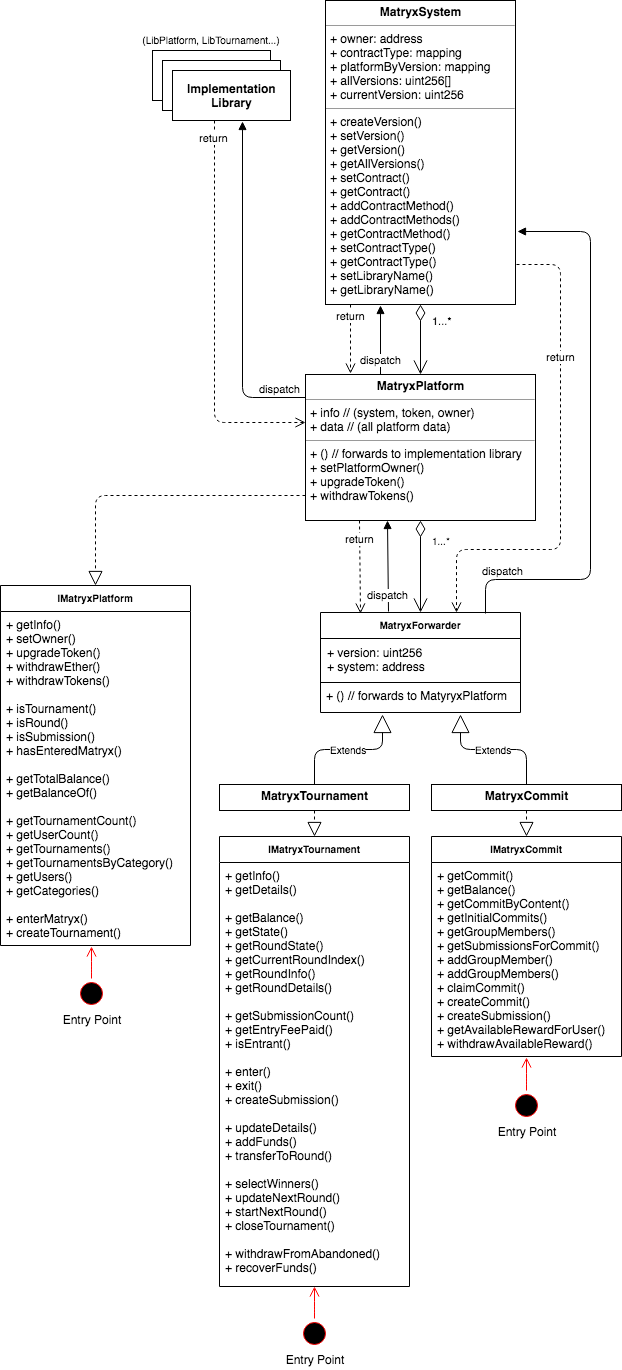
\includegraphics[scale = .5]{../Figures/MatryxArchitecture2018-MatryxPlatform.png}
\end{figure*}

\end{document}